\subsection{Drawing a 2D Lattice}
\paragraph{Learning Goals} We will be able to:
\begin{itemize}
	\item Draw a simple coordinate system (axes) using TikZ.
	\item Define vectors using \verb|\coordinate|.
	\item Generate lattice points using nested \verb|\foreach| loops.
	\item Label vectors and add mathematical captions.
\end{itemize}

\paragraph{What is a Lattice?}
Given two vectors $b_1,b_2 \in \mathbb{R}^2$, the \textbf{2D lattice generated by} $(b_1,b_2)$ is:
\[
\mathcal{L}(b_1,b_2)=\left\{x_1 b_1 + x_2 b_2 : x_1,x_2\in\mathbb{Z}\right\}.
\]
That means: start at the origin, move $x_1$ times along $b_1$ and $x_2$ times along $b_2$ (forward or backward),
and mark every point you can reach.
\begin{center}
\includegraphics[scale=1]{tikzs/2d-lattice.pdf}
\end{center}

\newpage
%----------------------------------------------------------
\paragraph{TikZ Idea (What are we drawing?)}
%----------------------------------------------------------
We will draw:
\begin{enumerate}
	\item A border rectangle (just to frame the figure).
	\item The $x$-axis and $y$-axis.
	\item Two basis vectors $b_1$ and $b_2$ from the origin.
	\item Points of the form $i b_1 + j b_2$ for integers $i,j$ in a small range.
	\item Labels and a formula under the diagram.
\end{enumerate}

\begin{lstlisting}
\begin{tikzpicture}[scale=0.9]

	% 1) draw a border box
	\draw[thick] (-7,-6) rectangle (7,6);
	
	% 2) draw x- and y-axes
	\draw[->, thick] (-6.5,0) -- (6.5,0);
	\draw[->, thick] (0,-5.5) -- (0,5.5);
	
	% 3) choose two basis vectors b1 and b2
	\coordinate (b1) at (2.5,0.2);
	\coordinate (b2) at (0.3,2.3);
	
	% 4) draw lattice points i*b1 + j*b2
	% (small range so it stays simple)
	\foreach \i in {-2,-1,0,1,2}{
		\foreach \j in {-2,-1,0,1,2}{
			\fill ({\i*2.5+\j*0.3},{\i*0.2+\j*2.3}) circle (1.2pt);
		}
	}
	
	% 5) draw the basis vectors as arrows from the origin
	\draw[->,thick] (0,0) -- (b1);
	\draw[->,thick] (0,0) -- (b2);
	
	% 6) label the vectors
	\node[blue!70!black, font=\large] at ($(b1)+(0.5,0)$) {$b_1$};
	\node[blue!70!black, font=\large] at ($(b2)+(0,0.3)$) {$b_2$};
	
	% 7) write the formula under the picture
	\node at (0,-7)
	{$\mathcal{L}(b_1,b_2)=\left\{\sum x_i b_i : x_i\in\mathbb{Z}\right\}$};

\end{tikzpicture}
\end{lstlisting}


\subsubsection{The TikZ environment}
\begin{itemize}
	\item \verb|\begin{tikzpicture}[scale=0.9]| starts the drawing.
	\item \verb|scale=0.9| shrinks the entire picture to 90\% of its original size.
\end{itemize}
	
\subsubsection{Step 1: Border rectangle}
\[
\verb|\draw[thick] (-7,-6) rectangle (7,6);|
\]
\begin{itemize}
	\item \verb|\draw| draws lines/shapes.
	\item \verb|[thick]| makes the line thicker.
	\item \verb|(-7,-6)| is the bottom-left corner.
	\item \verb|(7,6)| is the top-right corner.
	\item \verb|rectangle| draws the rectangle using these opposite corners.
\end{itemize}
	
\subsubsection{Step 2: Axes}
\[
\verb|\draw[->, thick] (-6.5,0) -- (6.5,0);|
\]
\[
\verb|\draw[->, thick] (0,-5.5) -- (0,5.5);|
\]
\begin{itemize}
	\item \verb|--| draws a straight line segment.
	\item \verb|->| adds an arrowhead at the end.
	\item The first line is the $x$-axis from $x=-6.5$ to $x=6.5$.
	\item The second line is the $y$-axis from $y=-5.5$ to $y=5.5$.
\end{itemize}
	
\subsubsection{Step 3: Defining basis vectors with \texttt{\textbackslash coordinate}}
\[
\verb|\coordinate (b1) at (2.5,0.2);|
\]
\[
\verb|\coordinate (b2) at (0.3,2.3);|
\]
\begin{itemize}
	\item \verb|\coordinate (name) at (x,y);| stores a point with a name.
	\item Here, \verb|(b1)| and \verb|(b2)| are two vectors from the origin.
	\item Geometrically:
	\[
	b_1=(2.5,0.2),\qquad b_2=(0.3,2.3).
	\]
\end{itemize}
	
\subsubsection{Step 4: Lattice points using nested loops}
The key idea is that every lattice point has the form:
\[
(i,j)\mapsto i\,b_1 + j\,b_2.
\]
We loop over integers $i$ and $j$:
\[
\verb|\foreach \i in {-2,-1,0,1,2}{ ... }|
\]
\[
\verb|\foreach \j in {-2,-1,0,1,2}{ ... }|
\]
Inside the loops:
\[
\verb|\fill ({\i*2.5+\j*0.3},{\i*0.2+\j*2.3}) circle (1.2pt);|
\]

\subsubsection{Step 5: Drawing the basis vectors}
\[
\verb|\draw[->,thick] (0,0) -- (b1);|
\qquad
\verb|\draw[->,thick] (0,0) -- (b2);|
\]
\begin{itemize}
	\item Because \verb|(b1)| and \verb|(b2)| are named coordinates,
	TikZ knows where to draw the arrows.
\end{itemize}
	
\subsubsection{Step 6: Label placement}
\[
\verb|\node[...] at ($(b1)+(0.5,0)$) {$b_1$};|
\]
\begin{itemize}
	\item \verb|\node at (point) {text};| places text.
	\item \verb|($(b1)+(0.5,0)$)| means ``start at \verb|b1| and shift right by 0.5''.
	\item This uses the \texttt{calc} library: \verb|\usetikzlibrary{calc}|.
\end{itemize}
	
\subsubsection{Step 7: Adding the lattice definition}
\[
\verb|\node at (0,-7) {$\mathcal{L}(b_1,b_2)=\cdots$};|
\]
\begin{itemize}
	\item This places a math formula below the box.
\end{itemize}

\newpage
\subsection{Drawing a Skew Lattice with Parallel Line Families}
%----------------------------------------------------------
\paragraph{Learning Goals}
%----------------------------------------------------------
After this lesson, you will be able to:
\begin{itemize}
	\item Use \verb|\def| to create adjustable parameters for a TikZ figure.
	\item Clip drawings to a rectangular window using \verb|\clip|.
	\item Use \verb|\foreach| loops to generate repeated geometric objects.
	\item Draw two families of dashed parallel lines determined by two basis vectors.
	\item Compute lattice points $i b_1 + j b_2$ using \verb|\pgfmathsetmacro|.
	\item Combine all elements into a clear lattice diagram with a circle highlight.
\end{itemize}

\begin{lstlisting}
\begin{tikzpicture}[scale=0.9]
	
	% ---- (A) parameters you can easily change ----
	\def\xmin{-8}
	\def\xmax{ 8}
	\def\ymin{-3}
	\def\ymax{ 3}
	
	% basis vectors (change these to change the slant)
	\def\bax{2.0}   % b1 = (bax, bay)
	\def\bay{0.6}
	\def\bbx{0.6}   % b2 = (bbx, bby)
	\def\bby{1.8}
	
	% circle radius
	\def\R{2.4}
	
	% ---- (B) border (optional) ----
	\draw[thick] (\xmin,\ymin) rectangle (\xmax,\ymax);
	
	% clip everything to the box
	\begin{scope}
		\clip (\xmin,\ymin) rectangle (\xmax,\ymax);
		
		% ---- (C) axes ----
		\draw[thick] (\xmin,0) -- (\xmax,0);
		\draw[thick] (0,\ymin) -- (0,\ymax);
		
		% ---- (D) dashed parallel lines (two directions) ----
		% Lines parallel to b1, shifted by multiples of b2
		\foreach \k in {-6,-5,...,6}{
			% a point on the line: k*b2
			\pgfmathsetmacro{\px}{\k*\bbx}
			\pgfmathsetmacro{\py}{\k*\bby}
			% draw long segment in direction b1 through that point
			\draw[gray, dashed]
			({\px-20*\bax},{\py-20*\bay}) -- ({\px+20*\bax},{\py+20*\bay});
		}
		
		% Lines parallel to b2, shifted by multiples of b1
		\foreach \k in {-6,-5,...,6}{
			% a point on the line: k*b1
			\pgfmathsetmacro{\qx}{\k*\bax}
			\pgfmathsetmacro{\qy}{\k*\bay}
			% draw long segment in direction b2 through that point
			\draw[gray, dashed]
			({\qx-20*\bbx},{\qy-20*\bby}) -- ({\qx+20*\bbx},{\qy+20*\bby});
		}
		
		% ---- (E) lattice points: i*b1 + j*b2 ----
		\foreach \i in {-6,-5,...,6}{
			\foreach \j in {-6,-5,...,6}{
				\pgfmathsetmacro{\x}{\i*\bax+\j*\bbx}
				\pgfmathsetmacro{\y}{\i*\bay+\j*\bby}
				\fill (\x,\y) circle (2.2pt);
			}
		}
		
		% ---- (F) red circle and blue center point ----
		\draw[red, very thick] (0,0) circle (\R);
		\fill[blue] (0,0) circle (3pt);
		
	\end{scope}
\end{tikzpicture}
\end{lstlisting}
\begin{center}
	\includegraphics[scale=1]{tikzs/2d-lattice2.pdf}
\end{center}

\subsubsection{Step 1: Parameters you can easily change}
This block defines variables:
\begin{itemize}
	\item Window limits: \verb|\xmin,\xmax,\ymin,\ymax|.
	\item Basis vector components:
	\[
	b_1=(\texttt{bax},\texttt{bay}),\qquad b_2=(\texttt{bbx},\texttt{bby}).
	\]
	\item Circle radius \verb|\R|.
\end{itemize}

\subsubsection{Step 2: Border box and Clipping to the box}
\[
\verb|\draw[thick] (\xmin,\ymin) rectangle (\xmax,\ymax);|
\]
This draws a rectangle that frames the picture.
\[
\verb|\clip (\xmin,\ymin) rectangle (\xmax,\ymax);|
\]
Clipping means: anything drawn outside the rectangle is not shown.
This is useful because we will draw \emph{very long} dashed lines; clipping keeps them neat.

%\newpage
\subsubsection{Step 3: Axes}
\[
\verb|\draw[thick] (\xmin,0) -- (\xmax,0);|
\qquad
\verb|\draw[thick] (0,\ymin) -- (0,\ymax);|
\]
These draw the $x$- and $y$-axes across the window.
(If you want arrowheads, use \verb|[->,thick]|.)

\subsubsection{Step 4: Dashed parallel lines (two families)}
This is the key geometric idea.

\subsubsection*{Family 1: Lines parallel to $b_1$}
For each integer $k$, we take a point $k b_2$:
\[
k b_2 = (k\,\texttt{bbx},\,k\,\texttt{bby})
\]
and draw a line through it in the direction of $b_1$.

In code:
\begin{itemize}
	\item Compute a point on the line:
	\[
	\verb|\px = k*\bbx|,\qquad \verb|\py = k*\bby|
	\]
	\item Draw a long segment in direction $b_1$:
	\[
	(p_x,p_y)\pm 20\,b_1
	\]
	The number 20 is chosen so the segment is long enough to cover the window.
\end{itemize}

\subsubsection*{Family 2: Lines parallel to $b_2$}
Similarly, for each integer $k$ we take a point $k b_1$ and draw a line in direction $b_2$.

\paragraph{Why do we need two families?}
Together, these two families form a skew ``grid'' aligned with the lattice basis directions.

\subsubsection{Step 5: Lattice points}
This part draws the lattice:
\[
(i,j)\mapsto i b_1 + j b_2.
\]
We compute coordinates:
\[
x = i\,\texttt{bax} + j\,\texttt{bbx},\qquad
y = i\,\texttt{bay} + j\,\texttt{bby}.
\]
Then we plot a small filled circle.

\paragraph{Why use \texttt{\textbackslash pgfmathsetmacro}?}
It stores computed numeric values (like \verb|\x| and \verb|\y|) so you can use them
cleanly in \verb|\fill (\x,\y)|.

%\newpage
\subsubsection{Step 6: Circle and center point}
\[
\verb|\draw[red, very thick] (0,0) circle (\R);|
\]
draws a circle of radius \verb|\R| centered at the origin.

\[
\verb|\fill[blue] (0,0) circle (3pt);|
\]
draws a blue dot at the origin.


\newpage
\subsection{Drawing Rooted Trees}
%----------------------------------------------------------
\paragraph{Learning Goals}
%----------------------------------------------------------
After this lesson, you will be able to:
\begin{itemize}
	\item Draw a rooted tree using TikZ’s \verb|child| syntax.
	\item Style edges and nodes using TikZ styles.
	\item Use different node shapes (circles and squares).
	\item Control spacing with \verb|level distance| and \verb|sibling distance|.
	\item Read and modify a tree structure by matching indentation to hierarchy.
\end{itemize}

\medskip

\begin{lstlisting}
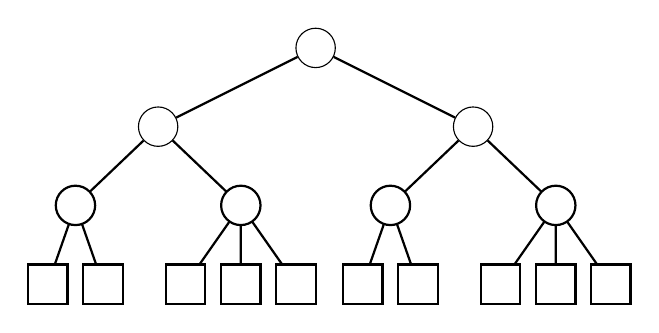
\begin{tikzpicture}[
	edge from parent/.style={draw, thick},
	every node/.style={draw, minimum size=5mm, inner sep=0pt},
	circ/.style={circle},
	sq/.style={rectangle},
	level distance=10mm,
	level 1/.style={sibling distance=40mm},
	level 2/.style={sibling distance=21mm},
	level 3/.style={sibling distance=7mm}
	]
	\node[circ] {}
	child { node[circ] {}
		child { node[circ] {}
			child { node[sq] {} }
			child { node[sq] {} }
		}
		child { node[circ] {}
			child { node[sq] {} }
			child { node[sq] {} }
			child { node[sq] {} }
		}
	}
	child { node[circ] {}
		child { node[circ] {}
			child { node[sq] {} }
			child { node[sq] {} }
		}
		child { node[circ] {}
			child { node[sq] {} }
			child { node[sq] {} }
			child { node[sq] {} }
		}
	};
\end{tikzpicture}
\end{lstlisting}
TikZ can draw trees using the pattern:
\[
\verb|\node {root} child { node {child1} } child { node {child2} };|
\]
\newpage
\begin{center}
	\includegraphics[scale=1]{tikzs/tree.pdf}
\end{center}

\paragraph{Key keywords}
\begin{itemize}
	\item \verb|\node ...;| creates the root node.
	\item \verb|child { ... }| creates a child subtree.
	\item Every \verb|child| contains another \verb|node|, which becomes the child node.
	\item Indentation is not required, but it helps you see the structure.
\end{itemize}

%----------------------------------------------------------
\subsubsection{Understanding the Style Block (The Part in [ ... ])}
%----------------------------------------------------------
At the top:\[
\verb|\begin{tikzpicture}[ ... ]|
\]
Everything inside \verb|[ ... ]| sets default styles and spacing.
\[
\verb|edge from parent/.style={draw, thick}|
\]
This means: every edge connecting a parent to a child is drawn as a thick line.
\[
\verb|every node/.style={draw, minimum size=5mm, inner sep=0pt}|
\]
This sets defaults for all nodes:
\begin{itemize}
	\item \verb|draw| draws the node border.
	\item \verb|minimum size=5mm| makes nodes at least 5mm in width/height.
	\item \verb|inner sep=0pt| removes extra padding inside nodes.
\end{itemize}
\[
\verb|circ/.style={circle}|
\qquad
\verb|sq/.style={rectangle}|
\]
These are \textbf{named styles} you can reuse:
\begin{itemize}
	\item \verb|node[circ]| makes a circular node.
	\item \verb|node[sq]| makes a rectangular node.
\end{itemize}
	
\newpage
%----------------------------------------------------------
\subsubsection{Spacing Control (Preventing Overlap)}
%----------------------------------------------------------
TikZ places nodes in levels (root at level 0, its children at level 1, etc.).
	
\[
\verb|level distance=10mm|
\]
This is the distance between one level and the next (vertical gap).
	
\[
\verb|level 1/.style={sibling distance=40mm}|
\]
\[
\verb|level 2/.style={sibling distance=21mm}|
\]
\[
\verb|level 3/.style={sibling distance=7mm}|
\]
\begin{itemize}
	\item \textbf{sibling distance} controls how far apart children of the same parent are.
	\item We give a larger distance near the top (level 1) because the big left and right subtrees
	must not overlap.
	\item Lower levels can use smaller distances because their subtrees are narrower.
\end{itemize}
	
%----------------------------------------------------------
\subsubsection{Reading the Tree Structure}
%----------------------------------------------------------
Start with the root:
\[
\verb|\node[circ] {}|
\]
This creates one circle (the root).
	
Then the root has \textbf{two children} because it has two \verb|child {...}| blocks:
\begin{itemize}
	\item First \verb|child {...}| is the left subtree.
	\item Second \verb|child {...}| is the right subtree.
\end{itemize}
	
\paragraph{Inside one subtree}
Example (left subtree):
\begin{lstlisting}
child { node[circ] {}
	child { node[circ] { ... } }
	child { node[circ] { ... } }
}
\end{lstlisting}
That means:
\begin{itemize}
	\item A circular node (level 1),
	\item with two circular children (level 2),
	\item each of which has several square leaves (level 3).
\end{itemize}

	
\newpage
\subsection{Building a One-Class SVM Figure with TikZ}
%----------------------------------------------------------
\paragraph{Learning Goals}
%----------------------------------------------------------
After this lesson, students should be able to:
\begin{itemize}
	\item Build a complex TikZ diagram using \textbf{structured blocks}.
	\item Use \verb|\def| parameters to control the picture (window size, origin position, slope, margin).
	\item Draw \textbf{axes} with an \textbf{off-center origin}.
	\item Plot lines defined by an equation (hyperplane and margins).
	\item Place points using \verb|\foreach| and basic coordinate arithmetic.
	\item Create annotated elements: arrows, labels, legend, and caption.
\end{itemize}
%The diagram is a common visualization for \textbf{one-class Support Vector Machines (SVM)}.
%It includes:
%\begin{itemize}
%	\item A feature space with axes $\Phi(x_1)$ and $\Phi(x_2)$.
%	\item A separating hyperplane (red solid line) and two margin boundaries (red dashed lines).
%	\item Training samples (black dots) representing the \emph{normal class}.
%	\item Support vectors (circled black dots) lying on/near the margin.
%	\item Samples violating the constraint (gray balls) labeled by slack variables $\xi_i,\xi_j$.
%	\item A legend explaining marker types.
%\end{itemize}

\begin{lstlisting}
\begin{tikzpicture}[scale=0.95, line cap=round, line join=round]
	
	% ----------------------------
	% 0) Canvas box
	% ----------------------------
	\def\xmin{-7} \def\xmax{7}
	\def\ymin{-7} \def\ymax{7}
	\draw[thick] (\xmin,\ymin-2) rectangle (\xmax,\ymax);
	
	% ----------------------------
	% 1) Off-center origin (like the figure)
	% ----------------------------
	\def\Ox{-2.4}
	\def\Oy{-1.2}
	\coordinate (O) at (\Ox,\Oy);
	
	\begin{scope}
		\clip (\xmin,\ymin) rectangle (\xmax,\ymax);
		
		% ----------------------------
		% 2) Axes
		% ----------------------------
		\draw[blue!70, very thick, ->] (\xmin+0.5,\Oy) -- (\xmax-1.5,\Oy)
		node[right] {$\Phi(x_1)$};
		\draw[blue!70, very thick, ->] (\Ox,\ymin+0.5) -- (\Ox,\ymax-1)
		node[above] {$\Phi(x_2)$};
		
		\fill[blue!80] (O) circle (4pt);
		\node[below left] at (O) {Origin};
		
		% ----------------------------
		% 3) Hyperplane + two margins (parallel)
		%    y - Oy = m(x - Ox) + c
		% ----------------------------
		\def\m{-1.05}   % slope
		\def\c{2.0}     % shift
		\def\dm{2}      % margin spacing
		
		% solid hyperplane
		\draw[red, very thick]
		(\xmin,{ \Oy + \m*(\xmin-\Ox) + \c }) --
		(\xmax,{ \Oy + \m*(\xmax-\Ox) + \c })
		node[pos=0.75, rotate=-46, black, above] {Optimal hyperplane};
		
		% dashed margins
		\draw[red, dashed, thick]
		(\xmin,{ \Oy + \m*(\xmin-\Ox) + \c + \dm }) --
		(\xmax,{ \Oy + \m*(\xmax-\Ox) + \c + \dm });
		
		\draw[red, dashed, thick]
		(\xmin,{ \Oy + \m*(\xmin-\Ox) + \c - \dm }) --
		(\xmax,{ \Oy + \m*(\xmax-\Ox) + \c - \dm });
		
		\node[rotate=-46] at (\Ox-3.5,\Oy+6.0) {$\textbf{w}\cdot \textbf{x} + b = 0$};
		
		% ----------------------------
		% 4) Margin arrow
		% ----------------------------
		\draw[gray, very thick, <->] (\Ox-1,\Oy+5) -- (\Ox-2.9,\Oy+3.1)
		node[gray!50!black, sloped, above, midway, font=\bfseries] {Margin};
		
		% ----------------------------
		% 5) w arrow
		% ----------------------------
		\draw[blue!70, very thick, ->] (\Ox+.5,\Oy+1.5) -- (\Ox+1,\Oy+2)
		node[sloped, above, midway] {$\textbf{w}$};
		
		% ----------------------------
		% 6) Normal class points (black cluster)
		% ----------------------------
		\foreach \p in {
			(0.9,4.1),(0.1,3.3),(1.7,3.4),(1.2,2.7),(0.4,2.6),
			(2.2,2.5),(0.5,1.9),(1.6,1.7),(2.5,1.7),(1.1,1.2),
			(2.1,1.1),(0.6,0.9),(1.5,0.5),(2.3,0.5),
			(1.2,1.9),(1.9,2.0)
		}{
			\fill \p circle (4pt);
		}
		
		% ----------------------------
		% 7) Support vectors (circled points)
		% ----------------------------
		\foreach \p in {(\Ox+2,\Oy+1.9), (\Ox+1,\Oy+2.9), (\Ox+3,\Oy+.9)}{
			\fill \p circle (4pt);
			\draw \p circle (7pt);
		}
		
		% ----------------------------
		% 8) Samples violating constraint (gray balls) + xi labels
		% ----------------------------
		\shade[ball color=gray!60] (\Ox+1,\Oy+.25) circle (5pt) node[above=2pt] {$\xi_i$};
		\shade[ball color=gray!60] (\Ox+1.75,\Oy-.5) circle (5pt) node[below=2pt] {$\xi_j$};
	\end{scope}
	
	% ----------------------------
	% 9) Legend box
	% ----------------------------
	\begin{scope}[shift={(0,-8)}]
		\draw[blue!60, fill=white, thick, rounded corners=4pt] (-4.5,-.75) rectangle (4.5,1.0);
		
		\fill (-4,0.5) circle (5pt) node[right=4pt] {Normal class};
		\draw (-.5,.5) circle (5pt) node[right=4pt] {Support vector};
		\shade[ball color=gray!60] (-.5,-0.25) circle (5pt) node[right=4pt] {Sample violating constraint};
	\end{scope}
	
	% ----------------------------
	% 10) Caption (optional)
	% ----------------------------
	\node at (0,-9.5) {Fig.\ 2.\quad One-class Support Vector Machine};
	
\end{tikzpicture}
\end{lstlisting}
\begin{center}
	\includegraphics[scale=.9]{tikzs/OCSVM.pdf}
\end{center}


\subsubsection{Block 0: Canvas box (plot window)}
\begin{itemize}
	\item The macros \verb|\xmin,\xmax,\ymin,\ymax| define the drawing window.
	\item The rectangle frames the figure:
\end{itemize}
\[
\verb|\draw[thick] (\xmin,\ymin-2) rectangle (\xmax,\ymax);|
\]
\textbf{Teaching tip:} Ask students why \verb|\ymin-2| is used (to make extra room for the legend/caption).

\subsubsection{Block 1: Off-center origin}
\[
\verb|\def\Ox{-2.4} \def\Oy{-1.2}|
\]
\[
\verb|\coordinate (O) at (\Ox,\Oy);|
\]
This is the most important design choice: the axes cross at (\verb*|\Ox|,\verb*|\Oy|) rather than $(0,0)$, matching the reference figure.

\subsubsection{Why we use \texttt{scope} + \texttt{clip}}
\[
\verb|\begin{scope} ... \clip ... \end{scope}|
\]
Everything inside this scope is clipped to the rectangle:
\begin{itemize}
	\item prevents lines and points from spilling outside,
	\item keeps the final graphic clean.
\end{itemize}

\subsubsection{Block 2: Axes with arrowheads and labels}
Key idea: use $(\verb*|\xmin|,\verb*|\Oy|)$ and $(\verb*|\Ox|,\verb*|\ymin|)$ to align axes with the off-center origin.

\[
\verb|(\xmin+0.5,\Oy) -- (\xmax-1.5,\Oy)|
\]
creates the horizontal axis across $y=\verb*|\Oy|$.

\[
\verb|(\Ox,\ymin+0.5) -- (\Ox,\ymax-1)|
\]
creates the vertical axis across $x=\verb*|\Ox|$.

\subsubsection{Block 3: Hyperplane and margins (equation-driven drawing)}
The hyperplane is defined by the shifted line equation:
\[
y - \verb*|\Oy| = m(x - \verb*|\Ox|) + c.
\]
So if we pick a value of $x$, TikZ computes $y$ by:
\[
y = \verb*|\Oy| + m(x-\verb*|\Ox|) + c.
\]
This is why the endpoints are written like:
\[
\verb|(\xmin,{ \Oy + \m*(\xmin-\Ox) + \c })|
\]

\paragraph{Margins.}
The dashed margins are parallel lines obtained by shifting $c$:
\[
c \to c+\mathrm{dm}\quad\text{and}\quad c\to c-\mathrm{dm}.
\]
In code, that is:
\[
\verb|... + \dm| \quad \text{and} \quad \verb|... - \dm|
\]

\subsubsection{Block 4: Margin arrow}
\[
\verb|\draw[gray, very thick, <->] (A) -- (B) node[...] {Margin};|
\]
\begin{itemize}
	\item \verb|<->| puts arrowheads on both ends.
	\item \verb|sloped| rotates the label to match the arrow direction.
	\item \verb|midway| puts the label in the middle.
\end{itemize}

\subsubsection{Block 5: The $\mathbf{w}$ direction arrow}
This arrow is a visual cue for the normal vector direction.
\[
\verb|(\Ox+.5,\Oy+1.5) -- (\Ox+1,\Oy+2)|
\]
Notice: these coordinates are written relative to $(\verb*|\Ox|,\verb*|\Oy|)$ so they move naturally if the origin moves.

\subsubsection{Block 6: Plotting the normal class points}
The code uses:
\[
\verb|\foreach \p in { (x1,y1),(x2,y2),... }{ \fill \p circle (4pt); }|
\]
This is the easiest way to plot many points:
\begin{itemize}
	\item Put point coordinates in the list.
	\item TikZ loops through them and plots each dot.
\end{itemize}

\subsubsection{Block 7: Support vectors (circled points)}
Support vectors are shown as a dot plus a surrounding circle:
\[
\verb|\fill \p circle (4pt);|
\quad \text{and} \quad
\verb|\draw \p circle (7pt);|
\]

\subsubsection{Block 8: Violating samples with shading}
The command:
\[
\verb|\shade[ball color=gray!60] (x,y) circle (5pt);|
\]
creates a nice “3D ball” effect. Then a node attaches the label $\xi_i$ or $\xi_j$.

\subsubsection{Block 9: Legend box}
The legend is drawn in a shifted scope:
\[
\verb|\begin{scope}[shift={(0,-8)}] ... \end{scope}|
\]
This moves the legend down without rewriting every coordinate.

Inside the legend, three marker types are drawn using:
\begin{itemize}
	\item \verb|\fill ... circle| for normal class,
	\item \verb|\draw ... circle| for support vectors (outline only),
	\item \verb|\shade ... circle| for violating samples.
\end{itemize}

%\subsubsection{Block 10: Caption}
%A simple \verb|\node| places the caption at a fixed coordinate.

%%----------------------------------------------------------
%\subsubsection{Parameters Students Can Experiment With}
%%----------------------------------------------------------
%Encourage students to change these and recompile:
%\begin{itemize}
%	\item \verb|\Ox,\Oy|: move the origin and see everything reposition correctly.
%	\item \verb|\m|: rotate the hyperplane (change slope).
%	\item \verb|\c|: shift the hyperplane up/down relative to the origin.
%	\item \verb|\dm|: widen/narrow the margin.
%	\item point coordinates: reshape the class distribution.
%\end{itemize}